\documentclass{mwrep}

% Polskie znaki
\usepackage{polski}
\usepackage[utf8]{inputenc}
\usepackage[T1]{fontenc}
\usepackage{lmodern}
\usepackage{indentfirst}

% Strona tytułowa
\usepackage{pgfplots}
\usepackage{siunitx}
\usepackage{paracol}

% Pływające obrazki
\usepackage{float}
\usepackage{svg}
\usepackage{graphicx}

% table of contents refs
\usepackage{hyperref}
\usepackage{cleveref}
\usepackage{booktabs}
\usepackage{listings}



\SendSettingsToPgf
\title{\bf Projekt układu regulacji obiektu grzejąco-chłodzącego\vskip 0.1cm}
\author{Krystian Guliński \and Jakub Sikora \and Konrad Winnicki}
\date{\today}
\pgfplotsset{compat=1.15}	
\begin{document}

\makeatletter
\renewcommand{\maketitle}{\begin{titlepage}
		\begin{center}{
				\LARGE {\bf Politechnika Warszawska}}\\
			\vspace{0.4cm}
			{\LARGE {\bf Wydział Elektroniki i Technik Informacyjnych}}\\
			\vspace{5cm}
			{\bf \LARGE \mbox{Systemy DCS i SCADA} \vskip 0.1cm}
		\end{center}
		\vspace{0.1cm}

		\begin{center}
			{\bf \LARGE \@title}
		\end{center}

		\vspace{10cm}
		\begin{paracol}{2}
			\addtocontents{toc}{\protect\setcounter{tocdepth}{1}}
			\subsection*{Zdający:}
			\bf{ \Large{ \noindent\@author \par}}
			\addtocontents{toc}{\protect\setcounter{tocdepth}{2}}

			\switchcolumn \addtocontents{toc}{\protect\setcounter{tocdepth}{1}}
			\subsection*{Prowadzący:}
			\bf{\Large{\noindent dr inż. Sebastian \\ Plamowski}}
			\addtocontents{toc}{\protect\setcounter{tocdepth}{2}}

		\end{paracol}
		\vspace*{\stretch{6}}
		\begin{center}
			\bf{\large{Warszawa, \@date\vskip 0.1cm}}
		\end{center}
	\end{titlepage}
}
\makeatother
\maketitle

\tableofcontents

\chapter{Obiekt regulacji}
\label{ObiektRegulacji}

\section{Opis obiektu termicznego}
\label{ObiektTermiczny}
Obiektem regulacji jest laboratoryjne stanowisko chłodząco-grzejące. Jest to obiekt cieplny, 
w którym jako elementy grzewcze wykorzystano rezystory mocy, w specjalnych obudowach dobrze odprowadzających
wytworzone ciepło. Do chłodzenia wykorzystano wysokoobrotowe
wentylatory. Zastosowano czujniki temperatury z magistralą danych
OneWire – oznaczenia. Dodatkowo wykorzystano płytę pomiarową
służącą do odczytu wartości prądu oraz napięcia. Urządzenie może pracować w trzech trybach komunikacji: poprzez
dedykowany protokół komunikacyjny przy użyciu standardu USB,
protokół MODBUS RTU oraz standard napięciowy RS485 lub poprzez
standard sygnałów analogowych 0-10V podłączając regulator przy użyciu złączy
śrubowych. Użytkownik ponadto ma możliwość zmiany charakteru obiektu, w tym celu
zamontowana została fizyczna przegroda. Wykorzystana jest ona do oddzielenia dwóch
strumieni powietrza wentylatora lewego i prawego, dzięki czemu można zredukować
zakłócenia wynikające z mieszania się strumieni. W ćwiczeniu, obiekt laboratoryjny
został znacząco uproszczony do przypadku jednowymiarowego. Wartością regulowaną była
wartość temperatury odczytana na czujniku temperatury T1. Sterowanie temperaturą odbywało się 
za pomocą grzałki G1. W ramach utrudnienia, na obiekt działało zakłócenie w postaci wentylatora W1.


\section{Proces modelowania obiektu}
\label{ModelowanieObiektu}
Przy pomocy zebranej odpowiedzi skokowej obiektu, za pomocą Matlaba dokonaliśmy identyfikacji 
modelu jednoinercyjnego. Pomimo że obiekt fizycznie jest co najmniej dwuinercyjny, zdecydowaliśmy się na 
przybliżenie go pojedynczą inercją w celu uproszczenia struktury regulacji. \\
\indent Do przeprowadzania identyfikacji wykorzystaliśmy funkcję \texttt{tfest}, która na podstawie 
przebiegów czasowych wyznacza parametry zadanej transmitancji. 

Otrzymany model obiektu:

\[model\_obiektu(s) = \frac{0.00395}{s + 0.008166}\]

\begin{figure}[H]
\centering
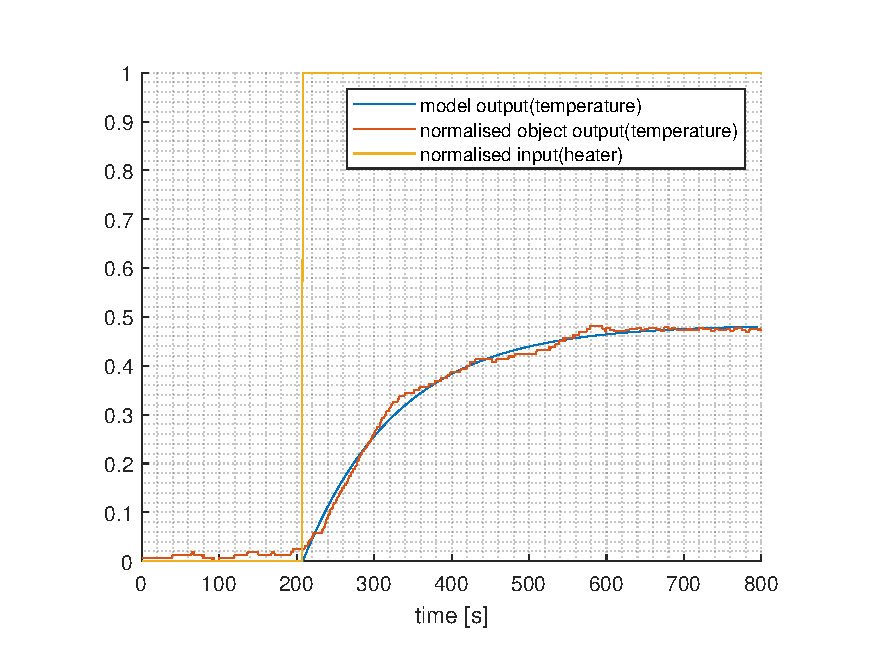
\includegraphics[scale=0.8]{materialy/krystian_plots/wykresik_model_obiekt.pdf}
\caption{Porownanie wyjscia modelu z obiektem}
\end{figure}

\section{Proces modelowania zakłóceń}
\label{ModelowanieZaklocen}
Przy pomocy zebranej odpowiedzi skokowej obiektu w trakcie reakcji na zmianę zakłóceń byliśmy w stanie w analogiczny sposób wyznaczyć również model zakłóceń, który potem będzie przydatny przy odsprzęganiu zakłóceń.

Otrzymany model zakłóceń:

\[model\_zaklocen(s) = \frac{-0.0003625}{s + 0.01105}\]

\begin{figure}[H]
\centering
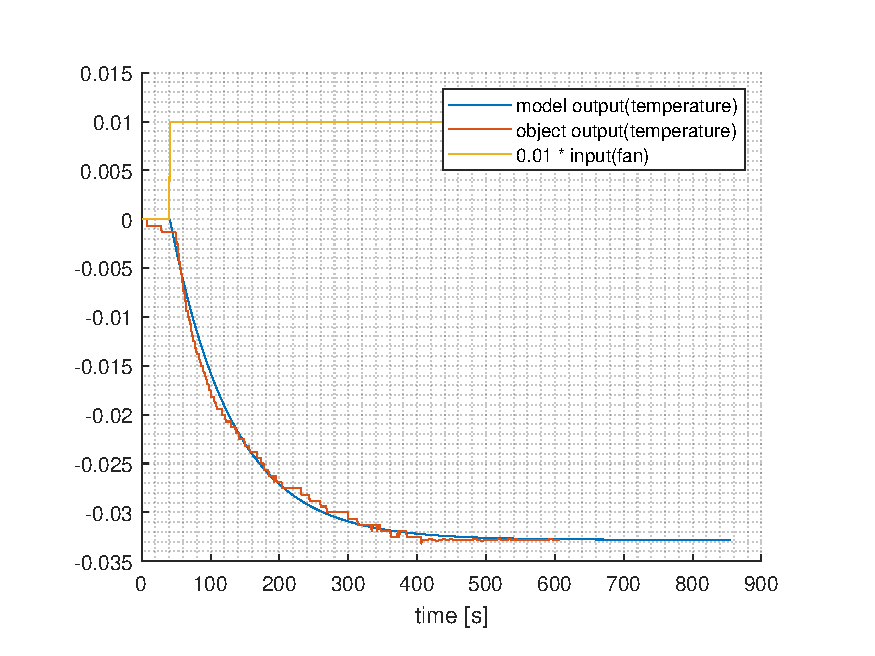
\includegraphics[scale=0.8]{materialy/krystian_plots/wykresik_zaklocenia.pdf}
\caption{Porownanie wyjscia modelu z obiektem w sytuacji badania zakłóceń}
\end{figure}

\section{Zebranie odpowiedzi skokowej}
\label{OdpowiedzSkokowa}

\chapter{Układ regulacji}
\label{UkladRegulacji}

\section{Opis struktury regulacji}
\label{OpisStruktury}

\subsection{Algorytm PID}
\label{PID}

Parametry regulatora PID zostały dobrane na podstawie modelu wyznaczonego w poprzedniej części projektu. W tym celu został użyty PID Tuner dostępny w środowisku MATLAB.

Równanie regulatora PIDF dostępnego w środowisku MATLAB:


$PIDF(s) = K _ { p } + \frac { K _ { i } } { s } + \frac { K _ { d } s } { T _ { f } s + 1 }$


Równanie regulatora PID dostępnego w systemie Ovation:

$PID\_OVATION(s) = K _ { p } + \frac { 1 } {  T _ { i } s } + \frac { K _ { d } s } { T _ { f } s + 1 }$

Jak widać różnica jest znikoma, aby dostosować parametry otrzymane z PID Tuner należy obliczyć wartość parametru Ti według wzoru

$T_{i} = \frac{1}{K_{i}}$

\begin{figure}[H]
\centering
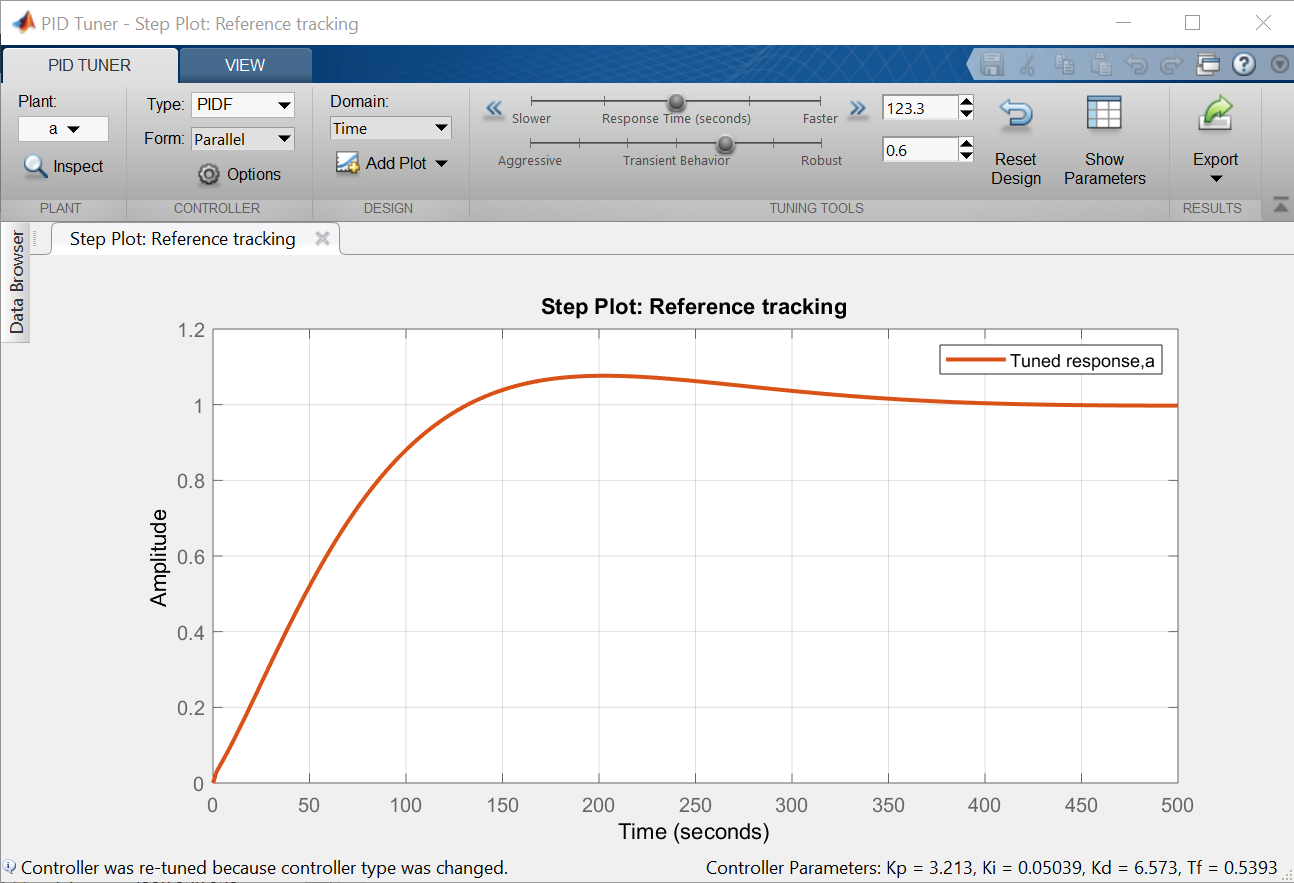
\includegraphics[scale=0.4]{materialy/krystian_plots/pid_tuner.png}
\caption{Widok procesu strojenia regulatora PID w PID Tunerze}
\end{figure}

Otrzymane parametry:

\begin{table}[]
\begin{tabular}{l|cccl}
Regulator    & Kp     & Ki/Ti        & Td     & Tf      \\ \hline
PIDF\_MATLAB & 3.2078 & Ki = 0.0502  & 6.3794 & 0.54035 \\
PID\_OVATION & 3.2079 & Ti = 19.8977 & 6.3794 & 0.54035
\end{tabular}
\end{table}





\subsection{Człon odsprzęgający}
\label{Odsprzeganie}

todo: trzeba wrzucić screena z ovation i opisać jak ten element ovationowy wpisane parametry zostały na podstawie tego modelu zakłóceń

\chapter{Implentacja w systemie OVATION}
\label{OVATION}

todo: Krystian: ja bym to wyrzucił ogólnie

\section{Control sheet}
\label{ControlSheet}

\section{Użyte algorymty}
\label{AlgorytmyOVATION}

\chapter{Testy układu regulacji}
\label{Testy}

\section{Testy wewnętrzne}
\label{TestyWewnetrzne}

\section{Konkurs grupowy}
\label{Konkurs}

\end{document}